\documentclass[conference]{IEEEtran}
\IEEEoverridecommandlockouts
% The preceding line is only needed to identify funding in the first footnote. If that is unneeded, please comment it out.
\usepackage{cite}
\usepackage{amsmath,amssymb,amsfonts}
\usepackage{algorithmic}
\usepackage{graphicx}
\usepackage{textcomp}
\usepackage{xcolor}
\usepackage{tabularx}
\usepackage{multirow}
\usepackage{graphics} % for pdf, bitmapped graphics files
\usepackage{subfig}
\usepackage{subcaption}
\usepackage{hyperref}
\usepackage{academicons}
\usepackage{xcolor}
\usepackage{listings}
\usepackage{tabularx} % Asegúrate de incluir este paquete

\usepackage{tikz}
\usetikzlibrary{shapes.geometric, arrows}

\usetikzlibrary{shapes.geometric, arrows}

\tikzstyle{startstop} = [rectangle, rounded corners, minimum width=3cm, minimum height=1cm,text centered, draw=black, fill=red!30]
\tikzstyle{process} = [rectangle, minimum width=3cm, minimum height=1cm, text centered, draw=black, fill=blue!30]
\tikzstyle{arrow} = [thick,->,>=stealth]


\def\BibTeX{{\rm B\kern-.05em{\sc i\kern-.025em b}\kern-.08em
		T\kern-.1667em\lower.7ex\hbox{E}\kern-.125emX}}

% Color Enlace
\definecolor{colorEnlace}{RGB}{0, 0, 0}
\hypersetup{
	colorlinks=true,
	linkcolor=colorEnlace,
	citecolor=colorEnlace,
	urlcolor=colorEnlace,
	pdfauthor={Davis Bremdow Salazar Roa},
	pdftitle={Sistemas Embebidos}
}
\definecolor{mybg}{rgb}{0.97,0.97,0.97}
\definecolor{mygray}{gray}{0.4}
\definecolor{mygreen}{rgb}{0,0.6,0}
\definecolor{myblue}{rgb}{0,0,0.8}
\definecolor{mypurple}{rgb}{0.58,0,0.82}
\definecolor{myred}{rgb}{0.7,0,0}

\lstdefinelanguage{MatlabEnhanced}{
	language=Matlab,
	morekeywords={[2]linspace,plot,title,xlabel,ylabel,legend,grid},
	morekeywords={[3]sin,cos,exp,log,sqrt},
	keywordstyle=\color{myblue}\bfseries,
	keywordstyle=[2]\color{mypurple},
	keywordstyle=[3]\color{myred},
	commentstyle=\color{mygreen}\itshape,
	stringstyle=\color{mygray},
	morecomment=[l]%
}

\lstset{
	language=MatlabEnhanced,
	backgroundcolor=\color{mybg},
	frame=single,
	basicstyle=\ttfamily\small,
	showstringspaces=false,
	numbers=none,              %
	xleftmargin=0pt,           %
	framexleftmargin=0pt,      
	framexrightmargin=0pt,
	framextopmargin=2pt,
	framexbottommargin=2pt,
	breaklines=true,
	tabsize=1,
}

% Control 
\usepackage{amsmath}
\begin{document}
	
	\title{Modulación FM - Análisis de una señal de voz}
	\author{
		\makebox[\textwidth][c]{\large\textbf{Universidad Nacional de San Antonio Abad del Cusco}}\\
		\makebox[\textwidth][c]{\normalsize\textit{Escuela profesional de Ingeniería Electrónica}}\\
		\makebox[\textwidth][c]{\normalsize\textit{Laboratorio de Circuitos Electrónicos III}}\\
		\and
		\IEEEauthorblockN{Ing. Milton Velasquez Curo}
		\IEEEauthorblockA{Ingeniero Electrónico \\
			Cusco, Perú \\
			milton.velasquez@unsaac.edu.pe}
		\and
		\IEEEauthorblockN{Ruth Juana Espino Puma - 185746}
		\IEEEauthorblockA{Estudiante de Ingeniería Electrónica \\
			Cusco, Perú \\
			184657@unsaac.edu.pe}
		\and
		\IEEEauthorblockN{Davis Bremdow Salazar Roa - 200353}
		\IEEEauthorblockA{Estudiante de Ingeniería Electrónica \\
			Cusco, Perú \\
			200353@unsaac.edu.pe}
	}
	
	\maketitle
	\begin{abstract}
		La modulación es un proceso fundamental en las telecomunicaciones que consiste en variar una o más propiedades de una señal portadora (como amplitud, frecuencia o fase) en función de una señal de información o mensaje. Este proceso permite transmitir información a largas distancias de manera eficiente, minimizando interferencias y aprovechando mejor el espectro de frecuencias. Existen varios tipos de modulación, entre ellos la modulación en amplitud (AM), frecuencia (FM) y fase (PM), cada una con características y usos específicos según las necesidades del sistema de comunicación.
		
	\end{abstract}
	
	\begin{IEEEkeywords}
		Modulación, portadora, señal, índice de modulación, amplitud, frecuencia, fase, transmisión, espectro, distorsión.
	\end{IEEEkeywords}
	
	%% Contenido del documento
	\section{Circuito Modulador FM}
	
	Una forma de poder implementar físicamente un modulador FM es mediante el empleo de circuito electrónicos, siendo uno de estos el circuito integrado XR2206 el cual es un generador de señales (sinusoidales, cuadradas y triangulares) según la configuración entre sus pines y las salidas a usar, un esquema genera sobre este integrado se puede obtener en su hoja de datos en la cual se detallan ejemplos y especificaciones sobre su funcionamiento.
	
	\begin{figure}[h]
		\centering
		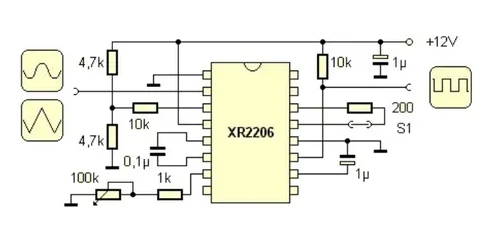
\includegraphics[width=0.5\textwidth]{media/integrado-xr2206}
		\caption{CI - Generador de señales XR2206}
		\label{fig:integrado-xr2206}
	\end{figure}
	
	En la figura \ref{fig:integrado-xr2206} se puede apreciar un esquema gráfico con una configuración inicial elegida para su funcionamiento como oscilador o generador de señales.
	
	Sin embargo si se desea tener un mayor control de la frecuencia de la señal generada el diagrama general del CI en la figura \ref{fig:diagrama-bloques-xr2206} muestra la configuración de pines, siendo los de relevancia los pines 5 y 6 (conexión para el capacitor) y 7 y 8 (pines para la resistencia) los cuales definen la frecuencia de oscilación del circuito bajo la ecuación que se define en \ref{eq:frecuencia-oscilacion} y utilizando el resto de pines para la polarización y salidas.
	
	Otra configuración a tener en cuenta corresponde a la amplitud de la portadora, la cual se puede configurar según la hoja de datos mediante la conexión entre los pines 13 y 14 para una señal senoidal y como un circuito abierto para el empleo de una señal triangulo, esta configuración a mayor detalle se aprecia en la figura \ref{fig:integrado-xr2206}, siendo necesario para modificar el valor de la resistencia entre ambos pines para modificar la amplitud la cual tiene una correspondencia proporcional entre el voltaje de salida respecto a la amplitud, donde se puede apreciar que se tendrá una salida de $a = \frac{60mV}{K\Omega}$, donde \textbf{a} representa la amplitud de la señal generada por el CI.
	
	\begin{equation}
		\omega_o = \frac{1}{CR}
		\label{eq:frecuencia-oscilacion}
	\end{equation}
	
	
	Una vez definidos los parámetros para el funcionamiento del CI, es posible tener un ejemplo sobre el funcionamiento del mismo mediante NI Multisim y en el cual este circuito se configurara de forma que sirva como un modulador FM mediante el empleo de una señal moduladora originada por el generador de funciones.
	
	\begin{figure}[h]
		\centering
		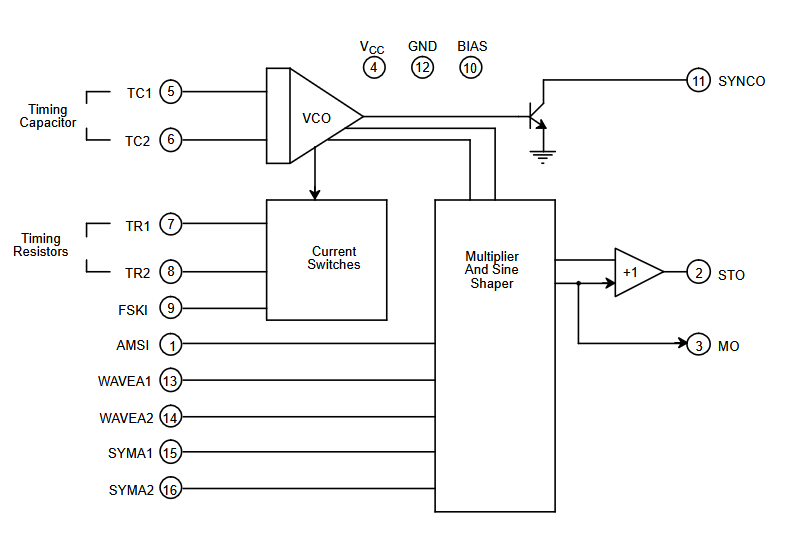
\includegraphics[width=0.5\textwidth]{media/diagrama-bloques-xr2206}
		\caption{Diagrama de bloques del CI XR2206}
		\label{fig:diagrama-bloques-xr2206}
	\end{figure}
	
	Un ejemplo de esta implementación se puede apreciar en la figura \ref{fig:simulacion-xr2206} en la cual se muestran los componentes antes mencionados para una frecuencia de la portadora de 1K Hz la cual responde a la inversa del producto de la capacitancia y resistencia según \ref{eq:frecuencia-oscilacion}.
	
	Mientras que el tono de información se configuro con una frecuencia de 100 Hz con un amplitud $V_{pp} = 20V$, la cual se acoplo al circuito integrado mediante un divisor de tensión al pin 7.
	
	
	\begin{figure}[h]
		\centering
		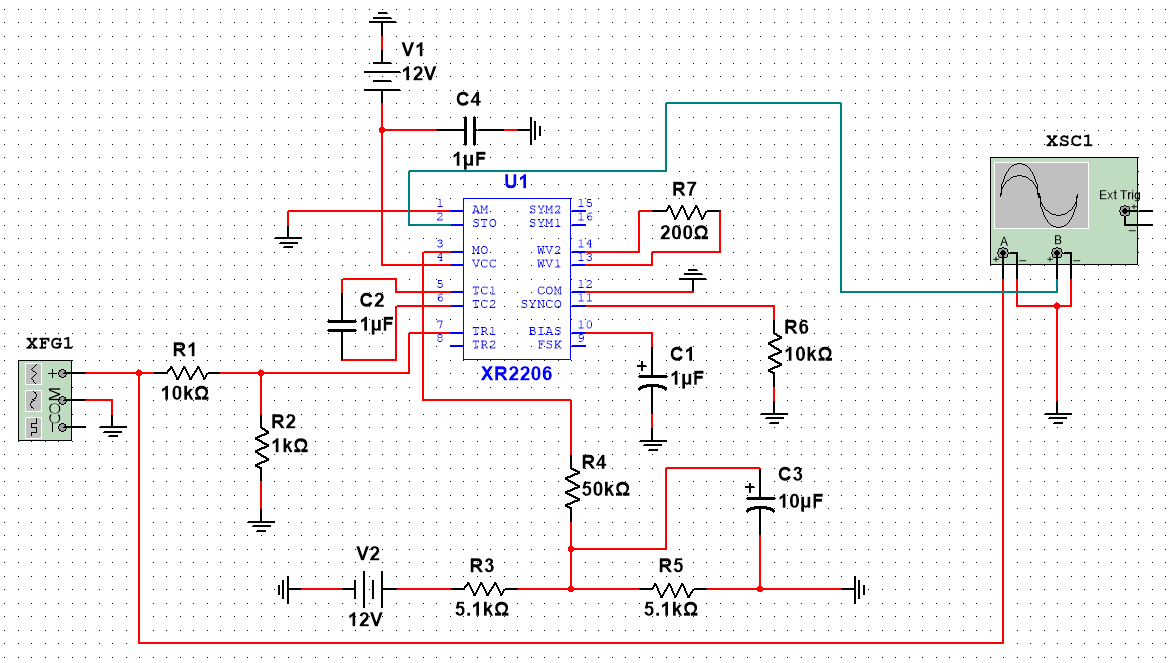
\includegraphics[width=0.5\textwidth]{media/simulacion-xr2206}
		\caption{Circuito Modulador FM - NI Multisim}
		\label{fig:simulacion-xr2206}
	\end{figure}
	
	Finalmente para la visualización de las señales se hizo uso de un osciloscopio de 2 entradas y en la cual se aprecia en su primer terminal la señal de información y en el segundo la señal FM generada a partir del CI XR2206 y mediante la cual se pudo apreciar las variaciones de frecuencia.
	
	\section{Señal FM generada}
	
	Mediante el empleo del osciloscopio se puede apreciar la forma de onda de salida del circuito integrado la cual al compararla con la señal sinuidal de entrada se puede apreciar los cambios de frecuencia para la excursión positiva de la señal como se muestra en la figura \ref{fig:mod-fm-circuito}.
	
	\begin{figure}[h]
		\centering
		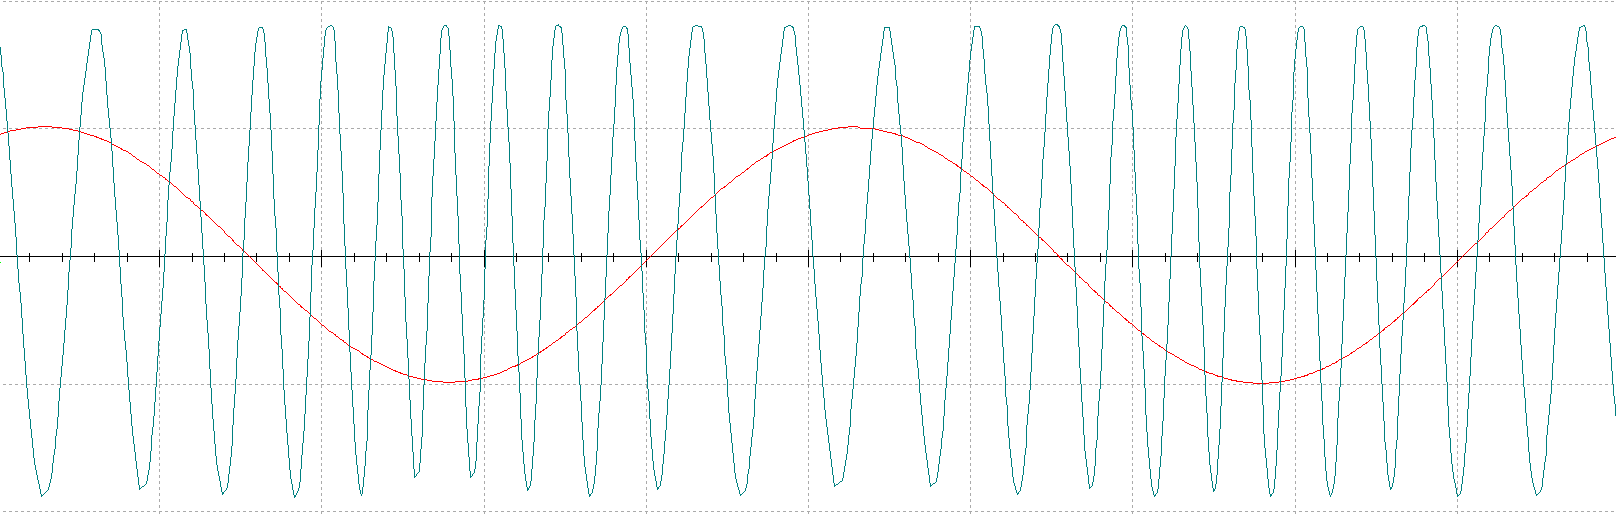
\includegraphics[width=0.5\textwidth]{media/mod-fm-circuito}
		\caption{Modulación FM - Circuito Integrado XR2206}
		\label{fig:mod-fm-circuito}
	\end{figure}
	
	Por otro lado si se considera una mayor frecuencia (400 [Hz]) en la moduladora, la señal de salida presenta cambios menos significativos en la señal, ello debido a que las variaciones de frecuencia son muy próximas a la frecuencia de la portadora, este efecto puede limitar la modulación debido a que se tendría una mezcla de señales muy parecida, este efecto se muestra en la figura \ref{fig:mod-fm-circuito-400}
	
	\begin{figure}[h]
		\centering
		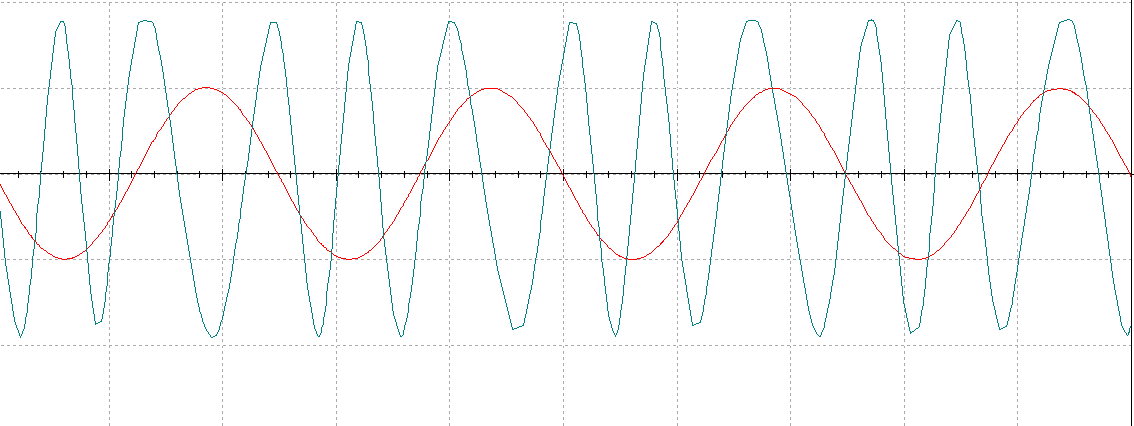
\includegraphics[width=0.7\textwidth]{media/mod-fm-circuito-400}
		\caption{Modulación FM de un tono - Circuito Integrado XR2206}
		\label{fig:mod-fm-circuito-400}
	\end{figure}
	
	
	\bibliographystyle{IEEEtran}
	\bibliography{biblio}
\end{document}
